\chapter{Good and bad modeling practices}
\label {ch15}

In preceding chapters, we reviewed the constructs from RDF, RDFS, and
OWL that go into a good model. We provided examples of successful models
from a number of different backgrounds. Even after reaching this point,
the prospect of creating a new model from scratch can seem daunting.
Where should you begin? How do you tell a good model from a bad one?

Unlike the examples in the previous chapters, many of the examples in
this chapter should not be

used as templates or examples of good practice in building your own
models. We indicate these examples with the label ``antipattern'' to
indicate patterns that should not be emulated in your models.

\section{Getting Started}

Often the first step of a journey is the most difficult one. How can you
start the construction of a useful semantic model? Broadly speaking,
there are three ways to get started, and the first comes directly from
the nature of a web. Why build something if it is already available on
the Web? One of the easiest ways to begin a modeling project is to find
models on the Web that suit your needs. The second way is to leverage
information assets that already have value for your organization.
It is not uncommon for an organization to have schemas, controlled
vocabularies, thesauri, or other information organization artifacts that
can provide an excellent source of vetted information
for a semantic model. The third way is to engineer a model from scratch.
In this case, certain standard engineering practices apply, including
the development of requirements definitions and test cases.

Regardless of the manner in which a model was acquired, you must answer
this question: Is this model, or some part of it, useful for my
purposes? This poses two issues for the modeler: How do I express my
intended purpose for a model? How do I determine whether a model
satisfies some purpose?

\subsection{Know what you want}

How can we express our intentions for the purpose of a model?  Since a model
is similar to other software artifacts (it is machine readable, and it drives our 
experience with information systems), we can borrow some insights from the conventional
wisdom of software engineering.  But models on the Semantic Web differ from many
software artifacts, so we need to understand how conventional software 
engineering practices
might fall short.

It is common in software engineering to speak of the 
requirements of a system we are about to build; what does the system have to 
do, given the state of the world in which it has to do it?  Starting from 
software requirements, there are a number of methodologies that guide software 
engineers in the construction of systems that satisfy those requirements. 

A model in the
Semantic Web goes beyond the usual role of an engineered artifact with
system requirements. On the Semantic Web, it is expected that a model
will be merged with other information, often from unanticipated sources.
This means that the design of a semantic model must not only respond to
known requirements, but also
express a range of variation that anticipates to some extent the
organization of the information with which it might be merged.

Although this seems like an impossible task (and in its full generality,
of course, it is
impossible to anticipate all the uses to which a model might be
applied), it is usually quite manageable. Take \texttt{ShakespeareanWork}
as an example.  Suppose that among your known requirements, you know that 
someone will want to sort through the works of Shakespeare, and perhaps
filter other questions by asking which results are also works of Shakespeare. 
In this case, it is pretty easy to know how to model \texttt{ShakespeareanWork}; it 
is a class, whose members are the works of Shakespeare. 
If you were working only with your own known requirements, then you would be
finished.  But on the web, people are interested in more things than Shakespeare.
If you were to anticipate that someone might be interested in all of the works
of the Elizabethan era (\texttt{ElizabethanWork}), then you would want to model not just
\texttt{ElizabethanWork} but also, and more importantly from an ontology modeling 
perspective, the relationship between \texttt{ElizabethanWork} and \texttt{ShakespeareanWork}.  Since the fact of the matter is that any \texttt{ShakespeareanWork} is also an \texttt{ElizabethanWork}, then you model the former as a \textt{subClassOf} the latter. 

This idea gets to the crux of how modeling in the Semantic Web differs
from many other engineering
modeling practices. Not only do you have to model for a particular
engineering setting but for a variety of anticipated settings, as well.
We have already seen examples of how this acts as a driving force behind
our models in the wild.

This simple example leaves open a number of issues; how do we know what our expectations 
for future application of our models will be?  How do we write down and manage
the requirements we have for these models?  These questions can be addressed to some 
extent with the use of  \emph{motivating scenarios} and \emph{competency
questions}. %FAB: ideally here we should add a reference to: 
\footnote{M. Uschold and Gruninger M. Ontologies: Principles, methods and applications. Knowledge Engineering Review, Vol. 11:2, 93-136, 1996. Also available as AIAI-TR-191 from AIAI, The University of Edinburgh}

Scenarios in software engineering are information-rich stories that  capture problems and 
wishes for a system to be designed, and they are used as the starting point to a software 
development project. Just as in the case for a software, the design of an ontology needs 
a clear specification of its purpose and scope, including an awareness of the 
stakeholders that might interact with it. Scenarios help us identify the goals and limits 
of such a development by clearly stating why the ontology is being built, what its 
intended uses are, and who are the stakeholders.

Scenarios are human-friendly short stories, and as such, they foster communication in 
natural language while capturing situation, context, stakeholders, problems and solutions 
with their associated vocabulary.  Scenarios in classical software engineering reveal two 
important aspects of the system to be designed, namely: 

\begin{itemize}
    \item the needs that are not covered by the existing solutions together with the vocabulary to express these needs, and
    \item the possible solutions to these problems that would be supported by the introduction of a new system. 
\end{itemize}

Both of these are important for the development of an ontology-based solution.  A scenario 
also provides context and stakeholders, making it possible to have some idea  of the scope 
of reuse of the ontology (or ontologies) to be developed.  

How can a scenario specify the requirements an ontology must satisfy?  The text of a 
motivating scenario introduces informal \emph{competency questions}; that is, questions 
that have to be answered by the ontology, in order to support the scenarios. 
These questions
place  requirements on the ontology to express both the needs and the results 
captured in the scenarios. Together, the motivating scenarios and competency 
questions help 
us scope the ontology in terms of completeness (the extent to which it covers the 
scenario), specificity (the extend to which specific terms of the scenario are captured), 
granularity (the extend to which terms are precisely defined), formality (the extend to 
which definitions are formalized) and reusability (the scope of situations in which the
ontology will continue to produce useful answers). 
Motivating scenarios and competency questions together  serve as 
sources, guides and constraints capturing at the same time the directions, domains, seed 
terms and boundaries for the ontology design. 

The utility of Scenario 
analysis does not end with ontology design.  Scenarios continue to provide input 
throughout the continued development of an ontology, as they are tested, refined, 
and reused. As we see how the ontology is being used and re-used, new scenarios will 
be discovered  
and existing scenarios will  be refined, managing an evolutionary process of
ontology maintenance. 
%FAB : end of new text to introduce motivating scenarios



\subsection{Say what you mean, mean what you say}
\label{ch15:swym}
The March Hare in Alice in Wonderland challenged Alice to say what she
means and mean what she says. This is good advice for anyone building a
model as well; the model is a set of statements that we ought to stand
behind, and a modeling language gives us a way to make those statements.
When we make a statement, we should mean it. If we have something to
say, we should find a way to express it in a modeling language. We can
only do this, if we have a way of knowing what statements in a modeling
language mean. It is fine to talk about scenarios,  stakeholders, variation, and
competency questions, but even when we do have a specific understanding
of the intent of a model, how can we even determine whether the model,
as constructed, meets that intention?

We can appeal to the intuition behind the names of classes and
properties, but this is problematic for a number of reasons. First is
the issue known as ``wishful naming.'' Just because someone has named a
class \texttt{ElizabethanWork} doesn't mean that it will contain all or even any
works that might deserve that name. Second is the issue of precision.
Just what did the modeler mean by \texttt{ElizabethanWork}? Is it a work created
by Queen Elizabeth or one that was created during her reign? Or perhaps
it is a work created by one of a number of prominent literary figures
(the \texttt{ElizabethanAuthors}), whose names we can list once and for all. To
determine whether a model satisfies some intent, we need an objective
way to know what a model means and, in the case of competency questions,
how a model can answer questions.

There are two ways a Semantic Web model answers questions. The first is
comparable to the way a database answers questions: by having the
appropriate data indexed in a way that can be directly accessed to
answer the question. If we answer the question ``What are the
Elizabethan literary works?'' this way, we would do so by having a class
called, say, \texttt{ElizabethanWork} and maintain a list of works as members of
that class.

This method for answering questions is fundamental to data management;
at some point, we have to trust that we have some data that are correct
or that are at least correct enough for our purposes. The special
challenge of semantic modeling comes when we need to model for
variability. How do we make sure that our answer to the question ``What
are the Shakespearean works?'' is consistent with the answer to ``What
are the Elizabethan works?'' (and how does this relate to the answer to
the question ``Who are the Elizabethan authors?''). This brings us to
the second way a semantic model can answer questions: through the use of
inferencing.

We can determine a model's answer to a particular question (or query)
through an analysis of inferencing. What triples can we infer based on
the triples that have already been asserted? This gives us more power to
say what we mean and mean what we say. What do I mean when I refer to a
\texttt{ShakespeareanWork}? If I mean that every \texttt{ShakespeareanWork} is an
\texttt{ElizabethanWork}, then I should say that \texttt{ShakespeareanWork} is a subclass
of \texttt{ElizabethanWork}. If furthermore I mean that an \texttt{ElizabethanWork} is one
that was created or performed by an \texttt{ElizfabethanAuthor} and that
\texttt{Shakespeare} is one of these authors, then I say by building a model that
entails the corresponding inferences (e.g., using \texttt{owl:someValuesFrom}, as 
outlined in Section~\ref{ch12.somevaluesfrom}).
Inferencing is the way I can tell whether what I have said is what I
mean---do the inferences the model entrails reflect the relationships
between concepts that I mean to express?

%\section{Modeling for Reuse}%

%One of the principal drivers in the creation of a semantic model is that
%it will be used by someone other than its designer in a new context that
%was not fully anticipated. If you are designing a model, you must
%consider the challenges the people using your model might face. How can
%you make this job easier for them?

\section{Good Naming Practices}

In Chapter~\ref{ch5}, we saw the importance of using HTTP URIs to refer to entities
on the Web of Data (just as we have been using HTTP URIs on the hypertext Web for decades).
It should come as no surprise that naming in a distributed system like the web
can have subtle effect. 

First, in Chapter~\ref{ch5} we discussed at length the impact of the choice of 
domain name for an HTTP URI.   We also discussed the distinction between \emph{slash} and 
\emph{hash} URIs (Section~\ref{hash-or-slash}).  But once we have got all of those details 
out of the way, there is still the question of how we should choose the \emph{local} names 
for our URIs. 

The local name for a URI is the part of the name after the final slash (for slash URIs) or 
after the hash (for hash URIs).  This is the name that appears in the QName for the URI. 
For example, the local name for \texttt{skos:broader}  (Section~\ref{ch11.semrel}) is 
\emph{broader}; the local name for \textt{wikidata:Q41176} (Section~\ref{dbpedia})is 
\emph{Q41176}. 

\subsection{Meaningful/Meaningless URIs?}

The first question we will consider is whether the local name should be meaningful
when read by a human being or not.  There are two basic approaches to this question: 

\begin{enumerate}
    \item \emph{Opaque local names} Local names for URIs are meaningless strings, usually numbers, that are guaranteed to be unique inside that namespace.  Examples are \texttt{wikidata:Q41176} (``building'') and \texttt{agrovoc:c\_4397} (``Livestock''). 
    \item \emph{Readable local names} Local names for URIs have names that are meaningful
    for a human reader.  Examples are \texttt{skos:broader}, \texttt{owl:someValuesFrom}, and \texttt{fibo-be-le-lp:LegalPerson}.
\end{enumerate}

As we can already see, both approaches have a strong pedigree in successful examples.  
What are the trade-offs, and how should you make your choice? 

\subsubsection{Advantages of Opaque local names}
This is a choice that was explicitly made by the wikimedia foundation for the names of the 
resources on wikidata, and also by the UN/FAO in AGROVOC (Section~\ref{ch11.skos}).  What
are the advantages? 

First, in both of these cases, there is a chance that the preferred name of the
entity might change, as we learn more about our domain.  The word ``building'' seems 
stable enough, but it does have synonyms in English, and as we see how this resource is
being used, we might find that one of the other words (structure, construction, 
erection, edifice, etc.) 
is more appropriate.  Whan we use opaque local names, this bit of maintenance is simple.  We remove the triple

\begin{lstlisting}
wikidata:Q41176  rdfs:label "building" .
\end{lstlisting}

and replace it with


\begin{lstlisting}
wikidata:Q41176  rdfs:label "structure" .
\end{lstlisting}

For the FAO, there was another consideration (which might also be a consideration 
for wikidata).. 
that the United Nations recognizes six official languages, and all 
UN documents must be simultaneously published in all six of these languages. 
Suppose that the UN had chosen a human-readable local name for \texttt{c\_4397}, which one
should it be?  Should it be \texttt{agrovoc:Livestock} or should it be 
\texttt{agrovoc:B\'etail}?  One could argue that both options are in violation of 
UN language guidelines.  Opaque names solve this question without any further 
discussion. 

Another reason to use opaque names is to avoid the fallacy of \emph{wishful naming} 
as described in Section~\ref{ch15:swym}.  If we don't give our URIs a readable name
we won't be tempted to believe that they mean something that the model doesn't 
express.  In the infrastructure of the Web, URIs are actually meaningless; it does
nobody a service to pretend that they have meaning. 

\subsubsection{Disadvantages of opaque names}

Despite the advantages listed above, opaque names remain unpopular among students 
and developers.  The reasons for this are pretty obvious; when you are reading this 
book, and I refer to \texttt{agrovoc:c\_4397}, the text has to annotate somewhere that this
refers to ``Livestock'' (as we did in the introduction to this very section).   

This problem carries on into engineering settings; if we view a model or a vocabulary with 
a resource like \texttt{agrovoc:c\_4397} in a tool for managing ontologies or 
vocabularies, we see a structure full of these meaningless references.  It 
is very difficult to review a model if you can't read any of the concepts. 

This disadvantage can be dealt with, of course, by using tools that are aware of this 
problem.  Most vocabulary tools have a mode in which resources are displayed based on 
their label.  For example,  since AGROVOC includes the triples


\begin{lstlisting}
agrovoc:c_4397   skos:prefLabel   "Livestock"@en , "B(*@\'e@*)tail"@fr .
\end{lstlisting}


a vocabulary tool can display this using that name.  It can even switch to use
\texttt{B\'etail} if the tool is internationalized to use French. 

But even this solution has its problems; the National Agriculture Library for the
United States also has a thesaurus, which has considerable common coverage with 
AGROVOC, and there is a resource in that vocabulary called "Livestock".  If 
we want to compare and contrast these vocabularies, and we use even a 
sophisticated  tool that 
is able to deal with preferred labels and various languages, how should it display the
fact that one resource is the AGROVOC version of Livestock and the other is
the NAL version of Livestock?  If we had meaningful local names, then this
problem would have been solved already by the QNames:  
\texttt{agrovoc:Livestock} vs. \texttt{NAL:Livestock}.

\subsubsection{Disadvantages of Meaningful Names}


A problem with human readable local names comes up when we consider what constitutes 
a legal HTTP URI.  Since these URIs are used for identifying resources on the web, and
the URIs themselves are sent across the web as identifiers, the web transport protocols 
have a lot to say about their format.  In particular, the local part of an HTTP URI 
is not allowed to have any of a set of special characters, which include parentheses, ampersands, and spaces. 

The most natural name for many entities contains these characters; for 
example, \texttt{agrovoc:c\_2018} is "dairy cattle".  If we try to make a 
readable URI from this,
then it will contain a blank, which is not allowed by the HTTP URI protocol.  There
are ways around this, but all of them require breaking the connection between the URI
and the preferred name.  The main issue here is that we are letting a transport
protocol (HTTP) have an influence on a human communication form (the name of 
a concept in a vocabulary). 

In FIBO, for historical reasons, the URI names have all been done as human readable names.
Furthermore, in the history of FIBO, some of the names have been changed.  For example, 
the technical term \emph{Juridical Person} refers to a legal entity that is not a real
human being; it is a legal fiction.  Many sources find this usage confusing (a definition
that says that some kind of person is not a person is likely to be confusing), so 
FIBO changed the preferred name of this concept to \emph{Legal Entity}, to remove 
that confusion.  This put FIBO into a bit of a puzzling situation; should they 
simply change the label of the resource, so that we have a triple that looks like 
this?

\begin{lstlisting}
fibo-be-le-lp:JuridicalPerson rdfs:label "Legal Entity" .
\end{lstlisting}


If we are trying to avoid confusion, this practice is not likely to help. 

If we change the URI, we get a triple like this:

\begin{lstlisting}
fibo-be-le-lp:LegalEntity rdfs:label "Legal Entity" .
\end{lstlisting}


which is more normal, but now we have another problem; what do we do about the applications
across the web who have made a reference to \texttt{fibo-be-le-lp:JuridicalPerson}?  
Now their references refer to no resource that FIBO defines, and their applications
will not find the data they expect.  For an international standard such as FIBO, this
is not an acceptable situation. 

FIBO seems to be caught between two unacceptable choices; have a confusing
practice of labeling, where a readable URI has a label which is not consistent
with the URI local name, or risk breaking any datasets or applications that refer to 
the former name.  

FIBO makes a compromise solution to this problem.  It retains the old URI (since 
other datasets might refer to it), but marks it as ``deprecated''.  Furthermore, it 
establishes the connection from the deprecated URI to the new one, 
using \texttt{owl:equivalentClass}.  Finally, any supplemental infomormation
(definitions, restrictions, inverses, etc.) are moved to the new URI.  In the case of 
this example, this results in the following triples: 

\begin{lstlisting}
fibo-be-le-lp:JuridicalPerson rdfs:label "juridical person" ;
     owl:deprecated true ;
     owl:equivalentClass fibo-be-le-lp:LegalEntity .
fibo-be-le-lp:LegalEntity a owl:Class ;
     rdfs:label "legal entity" ;
     rdfs:subClassOf fibo-be-le-lp:LegalPerson ;
     owl:disjointWith fibo-be-le-lp:LegallyCompetentNaturalPerson ;
     ...
\end{lstlisting}


This mitigates many of the issues with changing identity of meaningful URIs, in that 
it keeps consistent labels, it satisfies legacy users, and it allows FIBO to 
change the name of key concepts when necessary.  

The pro's and con's of these conventions do not make for a clear victor, which is 
why we see examples of all of these usages in successful open ontologies today.  
This analysis has covered most of the concerns to be considered when making a
decision for any particular project. 

\subsection{Naming Conventions}

In the common case in which meaningful URIs are used, there are some limitations
on the allowable names (as we saw above with embedded spaces).  This and other 
considerations have led to a set of \emph{de facto} conventions for how to build
local names for models in RDFS and OWL.  These conventions map more or less to conventions
for naming in XML and other web modeling languages, and are followed by the W3C
itself as well as throughout this book.

\begin{itemize}
\item \textbf{Name resources in CamelCase}: CamelCase is the name given to the style of
naming in which multiword names are written without any spaces but with
each word written in uppercase. We see this convention in action in W3C
names like rdfs:subClassOf and owl:InverseFunctionalProperty.

\item \textbf{Start class names with capital letters}: We see this convention in the
W3C class names \texttt{owl:Restriction} and \texttt{owl:Class}.

\item \textbf{Start property names with lowercase letters}: We see this convention in
the W3C property names rdfs:subClassOf and owl:inverseOf. Notice that
except for the first letter, these names are written in CamelCase.

\item \textbf{Start individual names with capital letters}: We see this convention at
work in the
\texttt{lit:Shakespeare} and \texttt{ship:Berengaria} examples in this book.

\item \textbf{Name classes with singular nouns}: We see this convention in the W3C
class names owl:DatatypeProperty and owl:SymmetricProperty and in the
examples in this book: lit:Playwright.
\end{itemize}


\subsection{Keeping track of classes and individuals}

One of the greatest challenges when designing a semantic model is
determining when something should be modeled as a class and when it
should be modeled as an individual. This issue arises especially when
considering a model for reuse because of the distributed nature of a
semantic model. Since a semantic model must respond to competency
questions coming from different stakeholders, it is quite possible that
one work practice has a tradition of considering something to be a
class, whereas another is accustomed to thinking of it as an instance.

As a simple example, consider the idea of an endangered species. For the
field zoologists who are
tracking the number of breeding pairs in the world (and in cases where
the numbers are very small, give them all names), the species is a class
whose members are the individual animals they are tracking. For the
administrator in the federal agency that lists endangered species, the
species is an instance to be put in a list (i.e., asserted as a member
of the class of endangered species) or removed from that list. The
designer of a single model who wants to answer competency questions from
both of these stakeholder communities is faced with something of a
challenge. This situation can often be modeled effectively using the
\emph{Class-Individual Mirror} pattern in Chapter\ref{ch11}.

Another source of difficulty arises from the flexibility of human
language when talking about
classes and instances. We can say that Shakespeare is an Elizabethan
author or that a poem is a literary work. In the first sentence, we are
probably talking about the individual called Shakespeare and his
membership in a particular class of authors. In the second, we are
probably talking about how one class of things (poems) relates to
another (literary works). Both of these sentences use the words ``is
a(n)'' to describe these very different sorts of relationships. In
natural languages, we don't have to be specific about which
relationships we mean. This is a drawback of using competency questions
in natural language: The question ``What are the types of literary
works?'' could be interpreted as a request for the individuals who are
members of the class LiteraryWork, or it could be asking for the
subclasses (types) of the class LiteraryWork. Either way of modeling
this could be considered a response to the question.

Although there is no hard and fast rule for determining whether
something should be modeled as an instance or a class, some general
guidelines can help organize the process. The first is based on the
simple observation that classes can be seen as sets of instances. If
something is modeled as a class, then there should at least be a
possibility that the class might have instances. If you cannot imagine
what instances would be members of a proposed class, then it is a strong
indication that it should not be modeled as a class at all. For example,
according to this guideline it is unlikely that we should use
a class to refer to the literary figure known as Shakespeare. After all,
given that we usually understand that we are talking about a unique
literary figure, what could possibly be the instances of the class
Shakespeare? If there is none, then Shakespeare should properly be
modeled as an instance.

If you can imagine instances for the class, it is a good idea to name
the class in such a way that the nature of those instances is clear.
There are some classes having to do with Shakespeare that one might want
to define. For example, the works of the bard, including 38 plays, 254
sonnets, 5 long poems, and so on could be a class of interest to some
stakeholder. In such a case, the name of the class should not simply be
Shakespeare but instead something like \texttt{ShakespeareanWork}. Considerable
confusion can be avoided in the design phase by first determining what
is to be modeled (the bard himself, his works, his family, etc.), then
deciding if this should be a class or an instance, and then finally
selecting a name that reflects this decision.

The second guideline has to do with the properties that describe the
thing to be modeled. Do you know (or could you know) specific values for
those properties or just in general that there is some value? For
instance, we know in general that a play has an author, a first
performance date, and one or more protagonists, but we know specifically
about \emph{The Tempest} that it was written by William Shakespeare, was
performed in 1611, and has the protagonist Prospero. In this case, \texttt{The
Tempest} should be modeled as an instance, and \texttt{Play} should be modeled as
a class. Furthermore, \emph{The Tempest} is a member of that class.

\subsection{Model testing}

Once we have assembled a model---either from designed components, reused
components, or components translated from some other source---how can we
test it? In the case where we have competency questions, we can start by
making sure it is possible to formulate these questions using the vocabulary of the model, 
and then, of course, confirming that it is able to answer them. 
More important, in the distributed setting
of the Semantic Web, we have to be able to determine (by analyzing the inferences that
the model entails) whether the model maintains consistent answers to possible
competency questions from multiple sources. We can also determine test
cases for the model and bases of unit tests that can be rerun every time the model evolves.. This is particularly important when reusing a
model. How does the model perform (i.e., what inferences can we draw
from it?) when it is faced with information that is not explicitly in
the scope of its design? In the analysis to follow, we will refer
generally to model tests---ways you can determine if the model satisfies
its intent.

\section{COMMON MODELING ERRORS}

In light of the AAA slogan (Anybody can say Anything about Any topic),
we can't say that anything is really a modeling error. In our experience
teaching modeling to scientists, engineers, content managers, and
project managers, we have come across a handful of modeling practices
that may be counterproductive for the reuse goals of a semantic model.
We can't say that the models are strictly erroneous, but we can say that
they do not accomplish the desired goals of sharing information about a
structured domain with other stakeholders.

We have seen each of the antipatterns described in the following in a
number of models. Here, we describe each one in turn and outline its
drawbacks in terms of the modeling guidelines just given. We have given
each of them a pejorative (and a rather fanciful) name as a reminder
that these are

antipatterns---common pitfalls of beginning modelers. Whenever possible,
we will also indicate good practices that can replace the antipattern,
depending on a variety of possible desired intents for the model.

\subsection{Rampant classism (antipattern)}

A common reaction to the difficult distinction between classes and
instances is simply to define everything as a class. This solution is
encouraged by most modeling tools, since the creation of classes is
usually the first primitive operation that a user learns. The temptation
is to begin by creating a class with the name of an important, central
concept and then extend it by creating more classes whose names indicate
concepts that are related to the original. This practice is also common
when a model has been created by automatic means from some other
knowledge organization source, like a thesaurus. A thesaurus makes much
less commitment about the relationship between terms than does a
semantic model between classes or between classes and individuals.

As an example, someone modeling Shakespeare and his works might begin by
defining a class called \texttt{Shakespeare} and classes called \texttt{Plays}, \texttt{Poems},
\texttt{Poets}, \texttt{Playwrights}, and \texttt{TheTempest}. Then, define a property (an
\texttt{owl:ObjectProperty}) called \texttt{wrote} and assert that \texttt{Shakespeare} wrote all
of these things by asserting triples like the following:

\begin{lstlisting}
:Playwrights :wrote :Plays .
:Poets :wrote :Poems .
:Shakespeare :wrote :Plays .
:ModernPlays rdfs:subClassOf :Plays .
:ElizabethanPlays rdfs:subClassOf :Plays .
:Shakespeare :wrote :TheTempest . 
:Shakespeare :wrote :Poems .
\end{lstlisting}

and perhaps even

\begin{lstlisting}
:TheTempest rdfs:subClassOf :Plays .
\end{lstlisting}

This seems to makes sense because, after all, \texttt{TheTempest} will show up
next to \texttt{Plays} in just about any ontology display tool. The resulting
model is shown in Figure~\ref{fig:ch15.01}


\begin{figure}
\centering
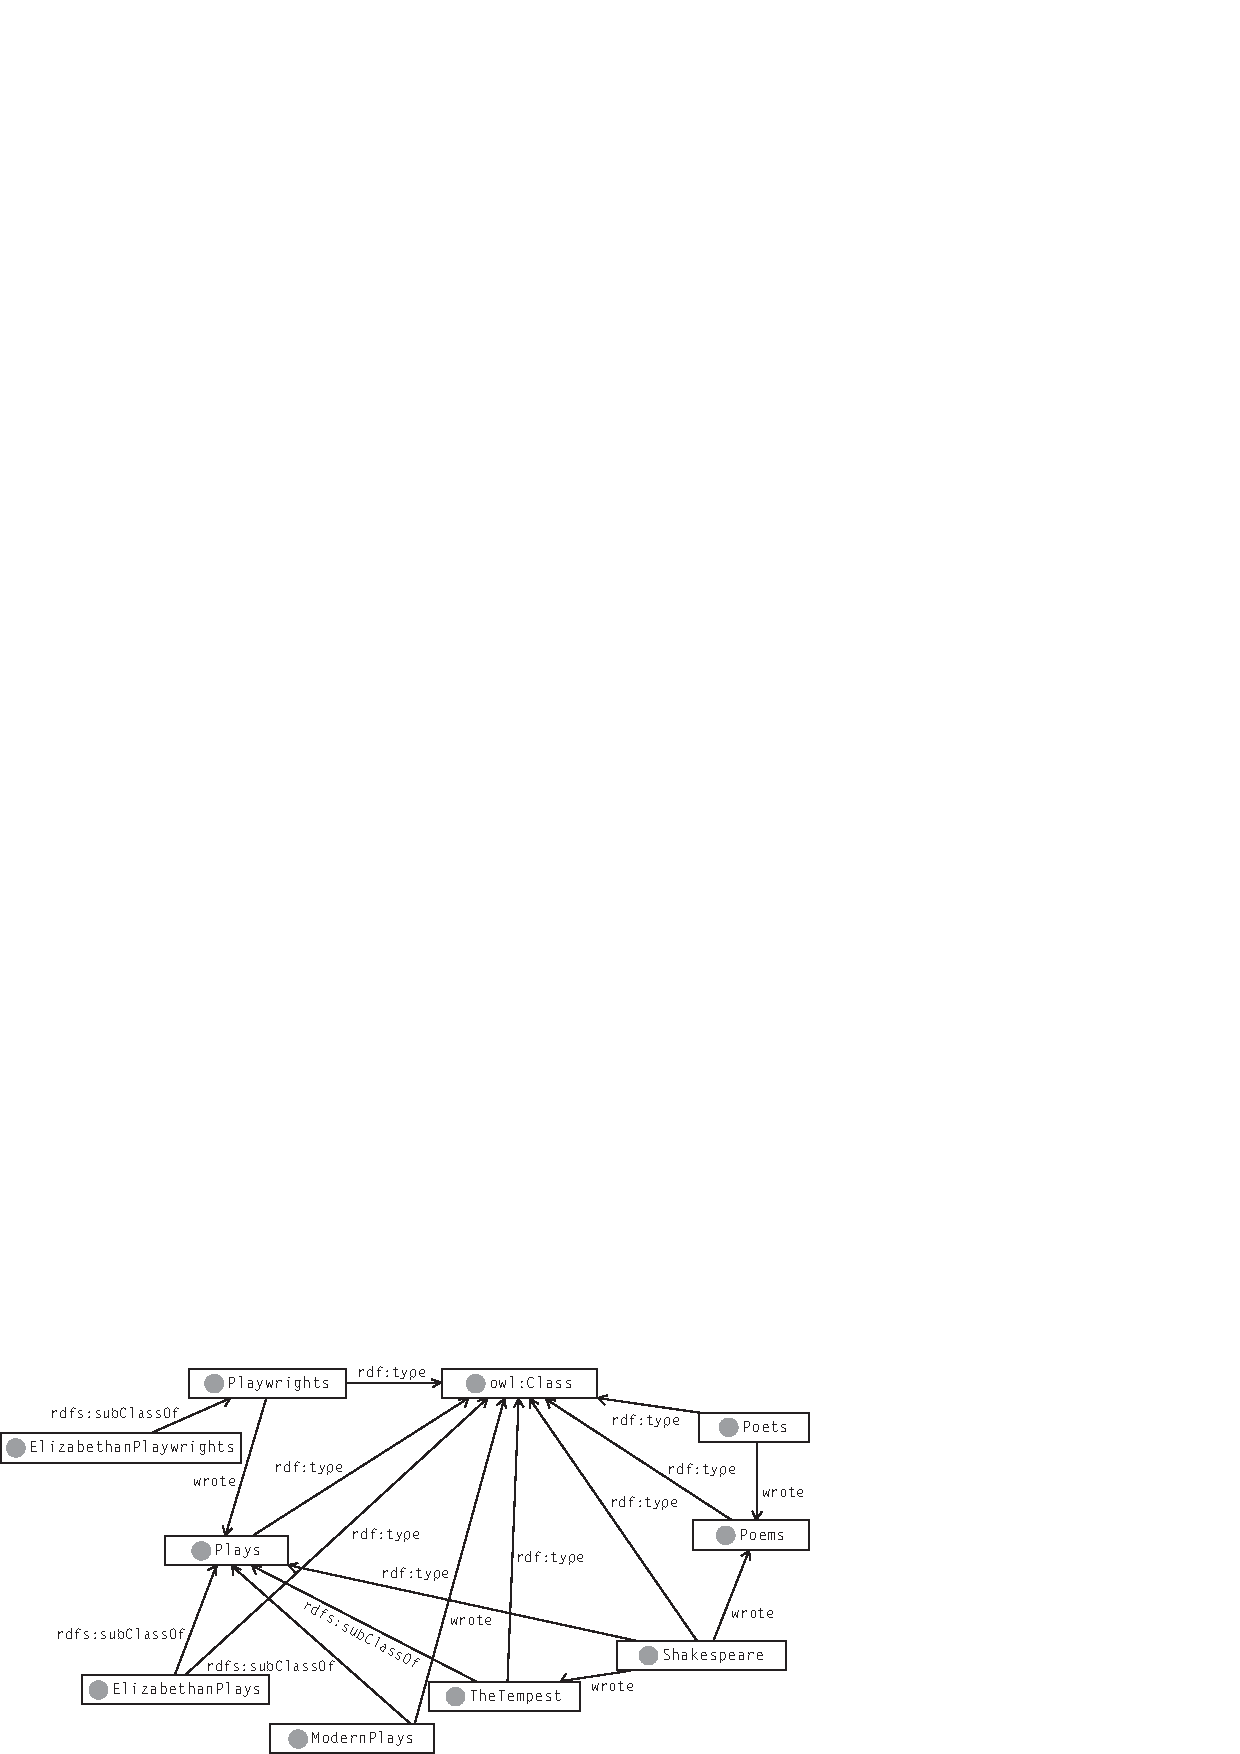
\includegraphics[width=5in]{media/ch15/f15-01.jpg}
\caption{Sample model displaying rampant classism. Every node in this model has
\texttt{rdf:type} \texttt{owl:Class}.
}
\label{fig:ch14.01}
\end{figure}


Given the AAA slogan, we really can't say that anything in this set of
triples is ``wrong.'' After all, anyone can assert these triples. But we
can start by noting that it does not follow the simple syntactic
conventions in that the class names are plurals.

This model reflects a style typical of beginning modelers. The triples
seem to translate into a sensible sentence in English: ``Shakespeare
wrote poems''; ``Shakespeare wrote The Tempest.'' If you render
\texttt{rdfs:subClassOf} in English as \emph{is a}, then you have ``The Tempest is a
plays,'' which aside from the plural at the end, is a reasonable
sentence in English. How can we evaluate whether this model satisfies
the intent of the modeler or of someone who might want to reuse this
model? We'll consider some tests that can tell us what this model might
be useful for.

Let's start with some simple competency questions. This model can
certainly answer questions of the form ``Who wrote The Tempest?'' The
answer is available directly in the model. It can also answer questions
like ``What type of thing writes plays? What type of thing writes
poems?'' Again, these answers are represented directly in the model.

Suppose we want to go beyond mere questions and evaluate how the model
organizes different points of view. It seems on the face of it that a
model like this should be able to make sure that the answer to a
question like ``What type of thing wrote Elizabethan plays?'' would at
the very least include the class of playwrights, since playwrights are
things that wrote plays and Elizabethan plays are plays. Can this model
support this condition? Let's look at the relevant triples and see what
inferences can be drawn:

\begin{lstlisting}
:Playwrights a owl:Class ;
             :wrote :Plays .
:ElizabethanPlays rdfs:subClassOf :Plays .
\end{lstlisting}

None of the inference patterns we have learned for OWL or RDFS applies
here. In particular, there is no inference of the form

\begin{lstlisting}
:Playwrights :wrote :ElizabethanPlays.
\end{lstlisting}

Another test criterion that this model might be expected to pass is
whether it can distinguish between plays and types of plays. We do have
some plays and types of plays in this model: \emph{The Tempest} is a play, and
Elizabethan play and modern play are types of plays. The model cannot
distinguish between these two cases. Any query that returns \emph{The Tempest}
(as a play) will also return modern plays. Any query that returns
Elizabethan play (as a type of play) will also return \emph{The Tempest}. The
model has not made enough distinctions to be responsive to this
criterion.

If we think about these statements in terms of the interpretation of
classes as sets, none of these results should come as a surprise. In
this model, playwrights and plays are sets. The statement
``Playwrights wrote plays'' makes no statements about individual
playwrights or plays; it makes a statement about the sets.

But sets don't write anything, whereas playwrights and poets do. This
statement, when made about sets, is nonsense. The OWL inference
semantics bear this out: The statement has no meaning, so no inferences
can be drawn. \texttt{TheTempest} is modeled here as a class, even though there
is no way to imagine what its instances might be; it is a play, not a
set. Plays are written by people (and have opening dates, etc.), sets do
not.

Similar comments can be made about a statement like ``Poets wrote
poems.'' If triples like:

\begin{lstlisting}
:Poets :wrote :Poems.
\end{lstlisting}

aren't meaningful, how should we render the intuition reflected by the
sentence ``Poets wrote poems''? This consideration goes beyond the
simple sort of specification that we can get from competency questions.
We could respond to questions like ``Which people are poets?'' or
``Which things are poems?'' with any model that includes these two
classes. If we want the answers to these two questions to have some sort
of consistency between them, then we have to decide just what
relationship between poems and poets we want to represent.

We might want to enforce the condition ``If someone is a poet, and he
wrote something, then it is a poem.'' When we consider the statement in
this form, it makes more sense (and a more readable model) if we follow
the convention that names classes with singular nouns (``a poet,'' ``a
poem'') rather than plurals (poets, poems).

We have already seen an example of how to represent a statement of this
form. If something is an \texttt{AllStarTeam}, then all of its players are
members of \texttt{StarPlayer}. Following that example, we can represent this
same thing about poets and poems as follows:

\begin{lstlisting}
:Poet rdfs:subClassOf [ a owl:Restriction;
                          owl:onProperty :wrote;
			  owl:allValuesFrom :Poem ] .
\end{lstlisting}

If we specify an instance of poet---say, Homer---and something he
wrote---say, \emph{The Iliad}---then we can infer that \emph{The Iliad} is a poem,
thus:

\begin{lstlisting}
:Homer :wrote :TheIliad .
:Homer a :Poet .
:TheIliad a :Poem .
\end{lstlisting}

This definition may work fine for Homer, but what happens if we press
the boundaries of the model a bit and see what inferences it can make
about someone like Shakespeare:

\begin{lstlisting}
:Shakespeare :wrote :TheTempest .
:Shakespeare a :Poet .
:TheTempest a :Poem .
\end{lstlisting}

The conclusion that \emph{The Tempest} is a poem is unexpected. Since it is
common for poets to write things that don't happen to be poems, probably
this isn't what we really mean by ``Poets wrote poems.'' This is an
example of a powerful method for determining the scope of applicability
of a model. If you can devise a test that might challenge some of the
assumptions in the model (in this case, the
assumption that nobody can be both a poet and a playwright), then you
can determine something about its boundaries.

What other results might we expect from the statement ``Poets wrote
poems''? We might expect that if someone is a poet, then they must have
written at least one poem. (We have already seen a number of examples of
this using \texttt{owl:someValuesFrom}.) In this case, this definition looks like
this:

\begin{lstlisting}
:Poet rdfs:subClassOf [a owl:Restriction ;
                       owl:onProperty :wrote ;
		       owl:someValuesFrom :Poem ].
\end{lstlisting}

The inferences we can draw from this statement are subtle. For instance,
from the following fact about Homer

\begin{lstlisting}
:Homer a :Poet .
\end{lstlisting}

we can infer that he wrote something that is a poem, though we can't
necessarily identify what it is.

When we say, ``Poets wrote poems,'' we might expect something even
stronger: that having written a poem is exactly what it means to be a
poet. Not only does being a poet mean that you have written a poem, but
also, if you have written a poem, then you are a poet. We can make
inferences of this sort by using \texttt{owl:equivalentClass} as follows:

\begin{lstlisting}
:Poet owl:equivalentClass [ a owl:Restriction;
                            owl:onProperty :wrote;
			    owl:someValuesFrom :Poem ] .
\end{lstlisting}

Now we can infer that Homer is a poet from the poem that he wrote

\begin{lstlisting}
:Homer :wrote :TheIliad .
:TheIliad a :Poem .
:Homer a :Poet .
\end{lstlisting}

In general, linking one class to another with an object property (as in
Poets wrote poems in this example) does not support any inferences at
all. There is no inference that propagates properties associated with a
class to its instances, or to its subclasses, or to its superclasses.
The only inferences that apply to object properties are those (like the
inferences having to do with \texttt{rdfs:domain} and \texttt{rdfs:range}, or inferences
from an \texttt{owl:Restriction}) that assume that the subject and object
(Shakespeare and poems in this case) are instances, not classes.

This illustrates a powerful feature of OWL as a modeling language. The
constructs of OWL make very specific statements about what the model
means, based on the inference standard. A sentence like ``Poets wrote
poems'' may have some ambiguity in natural language, but the
representation in OWL is much more specific. The modeler has to decide
just what they mean by a statement like ``Poets wrote poems,'' but OWL
allows these distinctions to be represented in a clear way.

\subsection{Exclusivity (antipattern)}

The rules of RDFS inferencing say that the members of a subclass are
necessarily members of a superclass. The fallacy of exclusivity is to
assume that the only candidates for membership in a subclass are those
things that are already known to be members of the superclass.

Let's take a simple example. Suppose we have a class called \texttt{City} and a
subclass called
OceanPort, to indicate a particular kind of city

\begin{lstlisting}
:OceanPort rdfs:subClassOf :City.
\end{lstlisting}

We might have a number of members of the class City, for example:

\begin{lstlisting}
:Paris a :City .
:Zurich a :City .
:SanDiego a :City .
\end{lstlisting}

According to the AAA assumption, any of these entities could be an
\texttt{OceanPort}, as could any other entity we know about---even things we
don't yet know are cities, like New York or Rio de Janeiro. In fact,
since Anyone can say Anything about Any topic, someone might assert that
France or The Moon is an \texttt{OceanPort}. From the semantics of RDFS, we would
then infer that France or The Moon are cities.

In a model that commits the error of exclusivity, we assume that because
\texttt{OceanPort} is a subclass of City, the only candidates for \texttt{OceanPort} are
those things we know to be cities, which so far are just Paris, Zurich,
and San Diego. To see how the exclusivity fallacy causes modeling
problems, let's suppose we are interested in answering the question
``What are the cities that connect to an ocean?'' We could propose a
model to respond to this competency question as follows:

\begin{lstlisting}
:OceanPort rdfs:subClassof :City.
:OceanPort owl:equivalentClass
     [ a owl:Restriction;
         owl:onProperty :connectsTo;
	 owl:someValuesFrom :Ocean ] .
\end{lstlisting}

These triples are shown graphically in Figure\ref{fig:ch15.02}

This model commits the fallacy of exclusivity; if we assume that only
cities can be ocean ports, then we can answer the question by querying
the members of the class \texttt{OceanPort}. But let's push the boundaries of
this model. What inferences does it draw from some boundary instances
that might violate some assumptions in the model? In particular, what if
we consider


\begin{figure}
\centering
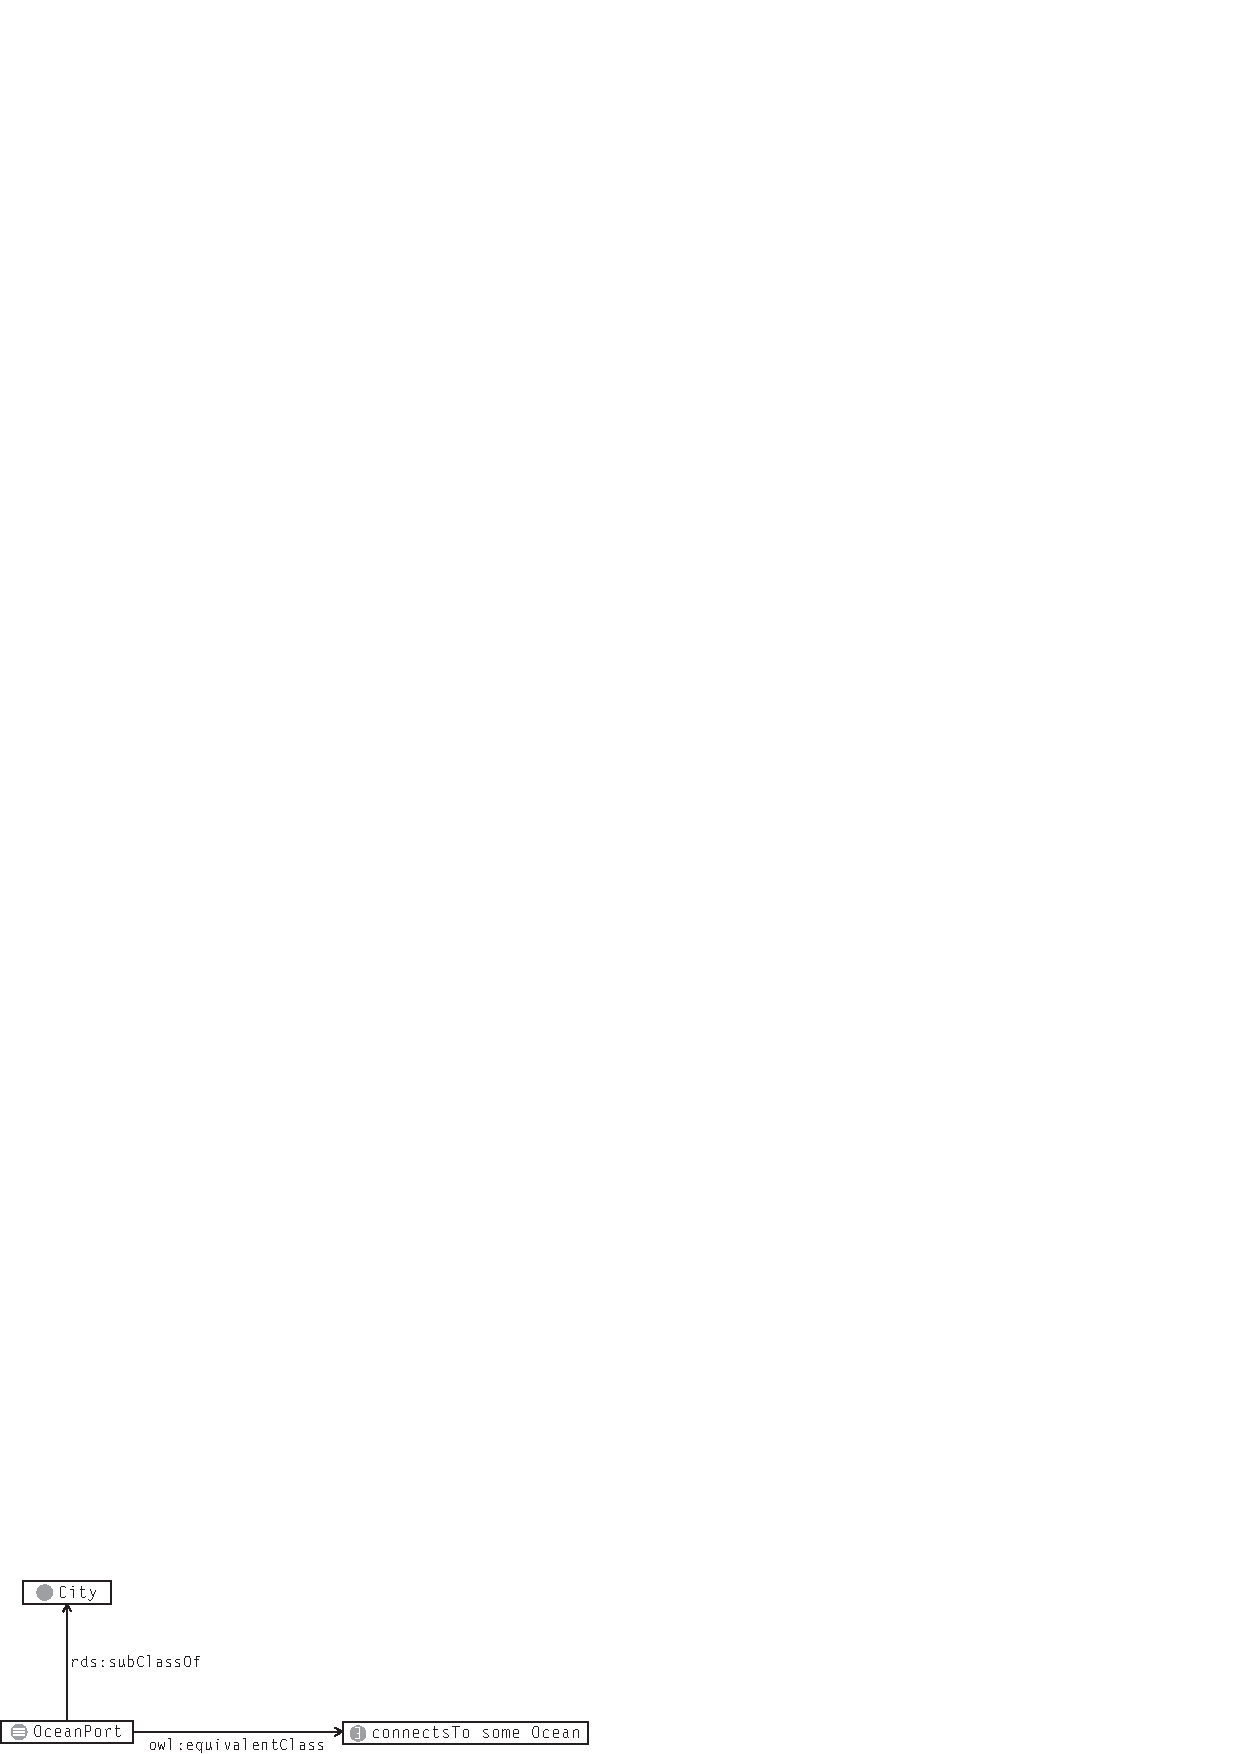
\includegraphics[width=5in]{media/ch15/f15-02.jpg}
\caption{Erroneous definition of OceanPort as a city that connects to an Ocean.}
\label{fig:ch15.02}
\end{figure}



something that is not a city but still connects to an ocean? Suppose we
have the following facts in our data set:

\begin{lstlisting}
:Zurich :connectsTo :RiverLimmat .
:Zurich :locatedIn :Switzerland .
:Switzerland :borders :France .
:Paris :connectsTo :LaSeine .
:Paris :locatedIn :France .
:France :connectsTo :Mediterranean .
:France :connectsTo :AtlanticOcean .
:SanDiego :connectsTo :PacificOcean .
:AtlanticOcean a :Ocean .
:PacificOcean a :Ocean .
...
\end{lstlisting}

From what we know about \texttt{SanDiego} and the \texttt{PacificOcean}, we can conclude
that
\texttt{SanDiego} is an \texttt{OceanPort}, as expected

\begin{lstlisting}
:SanDiego :connectsTo :PacificOcean .
:PacificOcean a :Ocean .
:SanDiego a :OceanPort .
\end{lstlisting}

Furthermore, since

\begin{lstlisting}
:OceanPort rdfs:subClassOf :City .
\end{lstlisting}

we can conclude that

\begin{lstlisting}
* :SanDiego a :City .
\end{lstlisting}

So far, so good, but let's see what happens when we look at France.

\begin{lstlisting}
:France :connectsTo :AtlanticOcean .
:AtlanticOcean a :Ocean .
\end{lstlisting}

Therefore, we can conclude that

\begin{lstlisting}
* :France a :OceanPort .
\end{lstlisting}

and furthermore,

\begin{lstlisting}
* :France a :City .
\end{lstlisting}

This is not what we intended by this model, and it does not respond
correctly to the question. The flaw in this inference came because of
the assumption that only things known to be cities can be ocean ports,
but according to the AAA assumption, anything can be an ocean port
unless we say otherwise.

This fallacy is more a violation of the AAA slogan than any
consideration of subclassing itself. The
fallacy stems from assumptions that are valid in other modeling
paradigms. For many modeling systems (like object-oriented programming
systems, library catalogs, product taxonomies, etc.) a large part of the
modeling process is the way items are placed into classes. This process
is usually done by hand and is called \emph{categorization} or \emph{cataloging}. The
usual way to think about such a system is that something is placed
intentionally into a class because someone made a decision that it
belongs there.



\begin{figure}
\centering
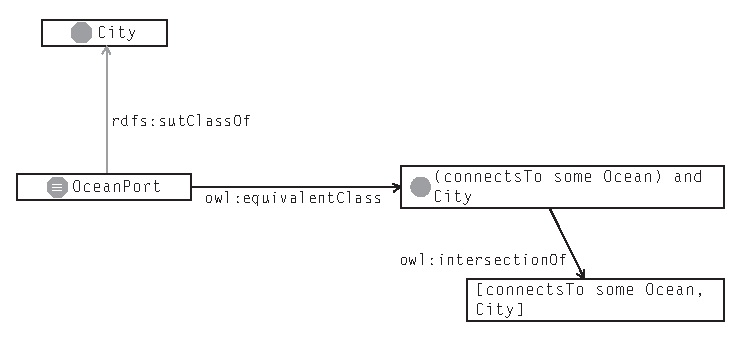
\includegraphics[width=5in]{SWWOv3/media/ch15/f15-03.eps}
\caption{Correct model for an OceanPort as a City that also connects to an Ocean.}
\label{fig:ch15.03}
\end{figure}



The interpretation of a subclass in this situation is that it is a
refinement of the class. If someone wants to make a more specific
characterization of some item, then they can catalog it into a subclass
instead of a class.

If this construct does not correctly answer this competency question,
what model will? We want something to become a member of OceanPort just
if it is both a City and it connects to an Ocean. We do this with an
intersection as shown in Figure~\ref{fig:ch15.03}.

Now that we have defined an \texttt{OcefanPort} as the intersection of \texttt{City} and a
restriction, we can infer that \texttt{OceanPort} is a subclass of \texttt{City}.
Furthermore, only individuals that are known to be cities are candidates
for membership in \texttt{OceanPort}, so anomalies like the previous one for
France cannot happen.

The Class Exclusivity fallacy is a common error for anyone who has
experience with any of a number of different modeling paradigms.
Semantic Web modeling takes the AAA assumption more seriously than any
other common modeling system. Fortunately, the error is easily remedied
by using the intersection pattern shown in Figure~\ref{fig:ch15.03}

\subsection{Objectification (antipattern)}

One common source of modeling errors is attempting to build a Semantic
Web model that has the same meaning and behavior as an object system.
Object systems, however, are not intended to work in the context of the
three Semantic Web assumptions: AAA, Open World, and Nonunique Naming.
In many cases, these differences in assumptions about the modeling
context result in basic clashes of modeling interpretation.

A fundamental example of this kind of clash can be found in examining
the role of a class in
a model. In object modeling, a class is basically a template from which
an instance is stamped. It makes little or no sense to speak of multiple
classes (stamped out of two templates?) or of having a property that
isn't in the class (where do you put it if there wasn't a slot in the
template for it?).

In Semantic Web models, the AAA and the Open World assumptions are
incompatible with this notion of a class. Properties in Semantic Web
models exist independently of any class, and because of the AAA slogan,
they can be used to describe any individual at all, regardless of which
classes it belongs to. Classes are seen as sets, so membership in
multiple classes is commonplace.

Let's consider a simple but illustrative example of how the intent of an
object model is incompatible with modeling in the Semantic Web. Suppose
an object model is intended to reflect the notion that a person has
exactly two parents who are also people. These are the requirements an
object model must satisfy:

\begin{enumerate}
\item A value for the property \texttt{hasParent} can be specified only for members
of the Person class.

\item  We will recognize as a mistake the situation in which only one value
for \texttt{hasParent} is specified for a single person.

\item  We recognize as a mistake the situation in which more than two values
for \texttt{hasParent} are specified for a single person.
\end{enumerate}


Before we even look at an OWL model that attempts to satisfy these
conditions, we can make some observations about the requirements
themselves. In particular, many of these requirements are at odds with
the fundamental assumptions of Semantic Web modeling, as described by
the AAA, Open World, and Nonunique Naming assumptions. Let's look at the
requirements in turn.

Requirement 1 is at odds with the AAA slogan. The AAA slogan tells us
that we cannot keep anyone from asserting a property of anything, so we
can't enforce the condition that hasParent can only be specified for
particular individuals. The Open World assumption complicates the
situation even further: Since the next thing we learn about a resource
could be that its type is Person, we can't even tell for sure whether
something actually is a person.

Requirement 2 is at odds with the Semantic Web assumptions. In this
case, the Open World assumption again causes problems. Just because we
have not asserted a second parent for any individual does not mean that
one doesn't exist. The very next Semantic Web page we see might give us
this information. Thus, regardless of how we model this in OWL, there
cannot be a contradiction in the case where too few parents have been
specified.

Requirement 3 is not directly at odds with the Semantic Web assumptions,
but the Nonunique Naming assumption makes this requirement problematic.
We can indeed say that there should be just two parents, so if more than
two parents are specified, a contradiction can be detected. This will
only happen in the case where we know that all the (three or more)
parents are distinct, using a construct like \texttt{owl:differentFrom},
\texttt{owl:allDifferent}, or \texttt{owl:disjointWith}.

The discrepancy between these requirements and an OWL model doesn't
depend on the details of
any particular model but on the assumptions behind the OWL language
itself. An object model is designed for a very different purpose from an
OWL model, and the difference is manifest in many ways in these
requirements.

Despite this mismatch, it is fairly common practice to attempt to model
these requirements in OWL. Here, we outline one such attempt and
evaluate the inference results that the model entails. Consider the
following model, which is a fairly common translation of an OO model
that satisfies these requirements into OWL:

\begin{lstlisting}
:Person a owl:Class .
:hasParent rdfs:domain :Person .
:hasParent rdfs:range :Person .
[ a owl:Restriction;
  owl:onProperty :hasParent;
  owl:Cardinality 2 ]
\end{lstlisting}

This model was created by translating parts of an object model directly
into OWL, as follows:

\begin{enumerate}
\item When a property is defined for a class in an OO model, that class is
listed as the domain of the property in OWL. The type of the property in
the OO model is specified as the range in OWL.

\item Cardinality limitations in the object model are represented by
defining a restriction class in OWL.
\end{enumerate}

We have already seen that this model cannot satisfy the requirements as
stated. How far off are we? What inference does this model support? What
inferences does it not support?

According to the stated intent of this model, if we assert just the
following fact:

\begin{lstlisting}
:Willem :hasParent :Beatrix .
\end{lstlisting}

The model should signal an error, since only a Person can have a parent,
and we have not asserted that Willem is a Person. If we fix this by
asserting that

\begin{lstlisting}
:Willem a :Person .
\end{lstlisting}

then the model should still indicate an error; after all, Willem must
have two parents, not just one. If we also assert more parents for
Willem:

\begin{lstlisting}
:Willem :hasParent :Claus .
:Willem :hasParent :TheDowager .
\end{lstlisting}

then the model should again signal an error, since now Willem has three
parents rather than two.

Now let's see what inferences can actually be made from these assertions
according to the inference patterns of OWL. From the very first
statement

\begin{lstlisting}
:Willem :hasParent :Beatrix .
\end{lstlisting}

along with the rdfs:domain information, we can infer that

\begin{lstlisting}
* :Willem a :Person .
\end{lstlisting}

That is, there is no need to assert that Willem is a Person before we
can assert who his parent is. This behavior is at odds with the first
intent; that is, we allowed Willem to have a parent, even though we did
not know that Willem was a person.

What about the cardinality restriction? What can we infer from that?
Three issues come into play with this. The first is the Open World
assumption. Since we don't know whether Willem might have another
parent, who simply has not yet been specified, we cannot draw any
inference about Willem's membership in the restriction. In fact, even if
we assert just one more parent for Willem (along with Beatrix, bringing
the total of asserted parents to exactly two) that

\begin{lstlisting}
:Willem :hasParent :Claus .
\end{lstlisting}

we still do not know that Willem really does have exactly two parents.
After all, there might be yet a third parent of Willem whom we just
haven't heard about. That's the Open World assumption.

The second issue has to do with unique naming. Suppose we now also
assert that

\begin{lstlisting}
:Willem :hasParent :TheDowager .
\end{lstlisting}

Surely, we can now infer that Willem cannot satisfy the restriction,
since we know of three parents, right? Even if there are more parents
lurking out there (according to the Open World assumption), we can never
get back down to just two. Or can we?

The Nonunique Naming assumption says that until we know otherwise, we
can't assume that two different names refer to different individuals. In
particular, the two names \texttt{TheDowager} and \texttt{Beatrix} could (and in fact, do)
refer to the same individual. So even though we have named three parents
for Willem, we still haven't disqualified him from being a member of the
restriction. We haven't named three distinct parents for Willem.

The third issue transcends all the arguments about whether Willem does
or does not satisfy the
cardinality restriction. Look closely at the definition of the
restriction: It is defined, as usual, as a bnode. If you read it aloud, it seems to say that the property \texttt{hasParent} has cardinality 2. But the bnode is not
connected to any other named class in any way. That is, the restriction
is not \texttt{owl:equivalentClass} to any other class, nor is it \texttt{rdfs:subClassOf}
any other class (or vice versa).

What does this mean for inferences involving this restriction? On the
one hand, even if we were to establish that Willem satisfies the
restriction, still no further inferences could be made. Further
inferences would have to be based on the connection of the restriction
to some other class, but there is no such connection. On the other hand,
if we could independently establish that Willem is a member of the
restriction, then we could possibly draw some conclusions based on that.
Since the restriction is not connected to any other class, there is no
independent way to establish Willem's membership in the restriction
class. Either way, we can draw no new inferences from this restriction.
The AAA slogan keeps us from saying that this model is ``wrong,'' but we
can safely say that it does not support the inferences that were
intended by the modeler. Unlike the case of the other anti- patterns, we
are not in a position to ``fix'' this model; the requirements of the
model are simply at odds with the assumptions of modeling in the
Semantic Web.

\subsection{Creeping conceptualization (antipattern)}

In most engineered systems, designing for reuse is enhanced by keeping
things simple. In software coding, for example, the best APIs try to
minimize the numbers of calls they provide. In physical systems, the
number of connections is minimized, and most common building materials
aim for a minimally constraining design so as to maximize the ways they
can be combined. On the Semantic Web, the same idea should apply, but
all too often the idea of ``design for reuse'' gets confused with ``say
everything you can.'' Thus, for example, when we include
\texttt{ShakespeareanWork} and \texttt{ElifzabethanWork} in our model, we are tempted to
further assert that \texttt{ElizabethanWork} is a subclass of \texttt{Work}, which is a
subclass of \texttt{IntangibleEntity}.

Of course, having included \texttt{IntangibleEntity}, you will want to include
\texttt{TangibleEntity} 
and some examples of those and some properties of those examples and,
well, \emph{ad infinitum}. After all, you might think that modeling for reuse
is best done by anticipating everything that someone might want to use
your model for, and thus the more you include the better. This is a
mistake because the more you put in, the more you restrict someone
else's ability to extend your model instead of just use it
as is. Reuse is best done, as in other systems, by designing to maximize
future combination with other things, not to restrict it.

This kind of creeping conceptualization may seem like an odd thing to
have to worry about. After all, isn't it a lot of extra work to create
more classes? Economists tell us that people minimize the amount of
unrewarded work they do. However, in practice, it often turns out that
knowing when to stop modeling is harder than deciding where to start. As
humans, we tend to have huge connected networks of concepts, and as you
define one class, you often think immediately of another you'd
``naturally'' want to link it to. This is an extremely natural tendency,
and even the best modelers find it very difficult to know when to
finish, but this way lies madness.

A relatively easy way to tell if you are going too far in your creation
of concepts is to check classes to see if they have properties
associated with them, and especially if there are restricted properties.
If so, then you are likely saying something useful about them, and they
may be included. If you are including data (instances) in your model,
then any class that has an instance is likely to be a good class. On the
other hand, when you see lots of empty classes, especially arranged in a
subclass hierarchy, then you are probably creating classes just in case
someone might want to do something with them in the future, and that is
usually a mistake. The famous acronym KISS (Keep It Simple, Stupid) is
well worth keeping in mind when designing Web ontologies.

\section{SUMMARY}

The basic assumptions behind the Semantic Web---the AAA, Open World, and
Nonunique Naming assumptions---place very specific restrictions on the
modeling language. The structure of RDF is in the form of statements
with familiar grammatical constructs like subject, predicate, and
object. The structure of OWL includes familiar concepts like class,
subClassOf, and property. But the meaning of a model is given by the
inference rules of OWL, which incorporate the assumptions of the
Semantic Web. How can you tell if you have built a useful model, one
that conforms to these assumptions? The answer is by making sure that
the inferences it supports are useful and meaningful.

According to the AAA slogan, we cannot say that any of the practices in
this chapter are ``errors'' because Anyone can say Anything about Any
topic. All of these models are valid expressions in RDF/ OWL, but they
are erroneous in the sense that they do not accomplish what the modeler
intended by creating them. In each case, the mismatch can be revealed
through careful examination of the inferences that the model entails. In
some cases (like the objectification error), the requirements themselves
are inconsistent with the Semantic Web assumptions. In other cases (like
the exclusivity error), the requirements are quite consistent with the
Semantic Web assumptions and can be modeled easily with a simple
pattern.

\subsection{Fundamental concepts}

The following concepts were introduced or elaborated in this chapter.

The Semantic Web Assumptions---AAA (Anyone can say Anything about Any
topic), Open- World, and Nonunique Naming.

Inferencing---In OWL, inferencing is tuned to respect the Semantic Web
assumptions. This results in subtleties that can be misleading to a
novice modeler.

Competency Questions---Questions that scope the requirements for a
model.

Modeling for Variability---The requirement (characteristic of Semantic
Web modeling) that a model describe variation as well as commonality.

Modeling for Reuse---The craft of designing a model for uses that cannot
be fully anticipated.

Wishful Naming---The tendency for a modeler to believe that a resource
signifies more than the formal semantics of the model warrants, purely
on the basis of the resource's name.

Model Testing---A process by which the boundaries of a model are
stressed to determine the nature of the boundaries of the inferences it
can entail.

